\subsubsection{Referee Login}

\textbf{Role:} Race Referee

\begin{itemize}
    \item \textbf{Function trigger:} The referee enters account credentials to log in.

    \item \textbf{Function description:}
    \begin{itemize}
        \item \textbf{Purpose:}
        \begin{enumerate}
            \item Verify the referee's identity.
            \item Grant access to referee functionalities.
        \end{enumerate}

        \item \textbf{Data processing:}
        \begin{enumerate}
            \item The referee enters username and password.
            \item The system validates credentials.
            \item The system identifies the REFEREE role.
            \item The system creates a login session.
        \end{enumerate}
    \end{itemize}

    \item \textbf{Function details:}
    \begin{itemize}
        \item Successful login redirects to Referee Dashboard.
        \item Invalid credentials display an error message.
        \item Users without accounts may register.
    \end{itemize}
\end{itemize}

\textbf{Screen layout:}

\begin{figure}[H]
    \centering
    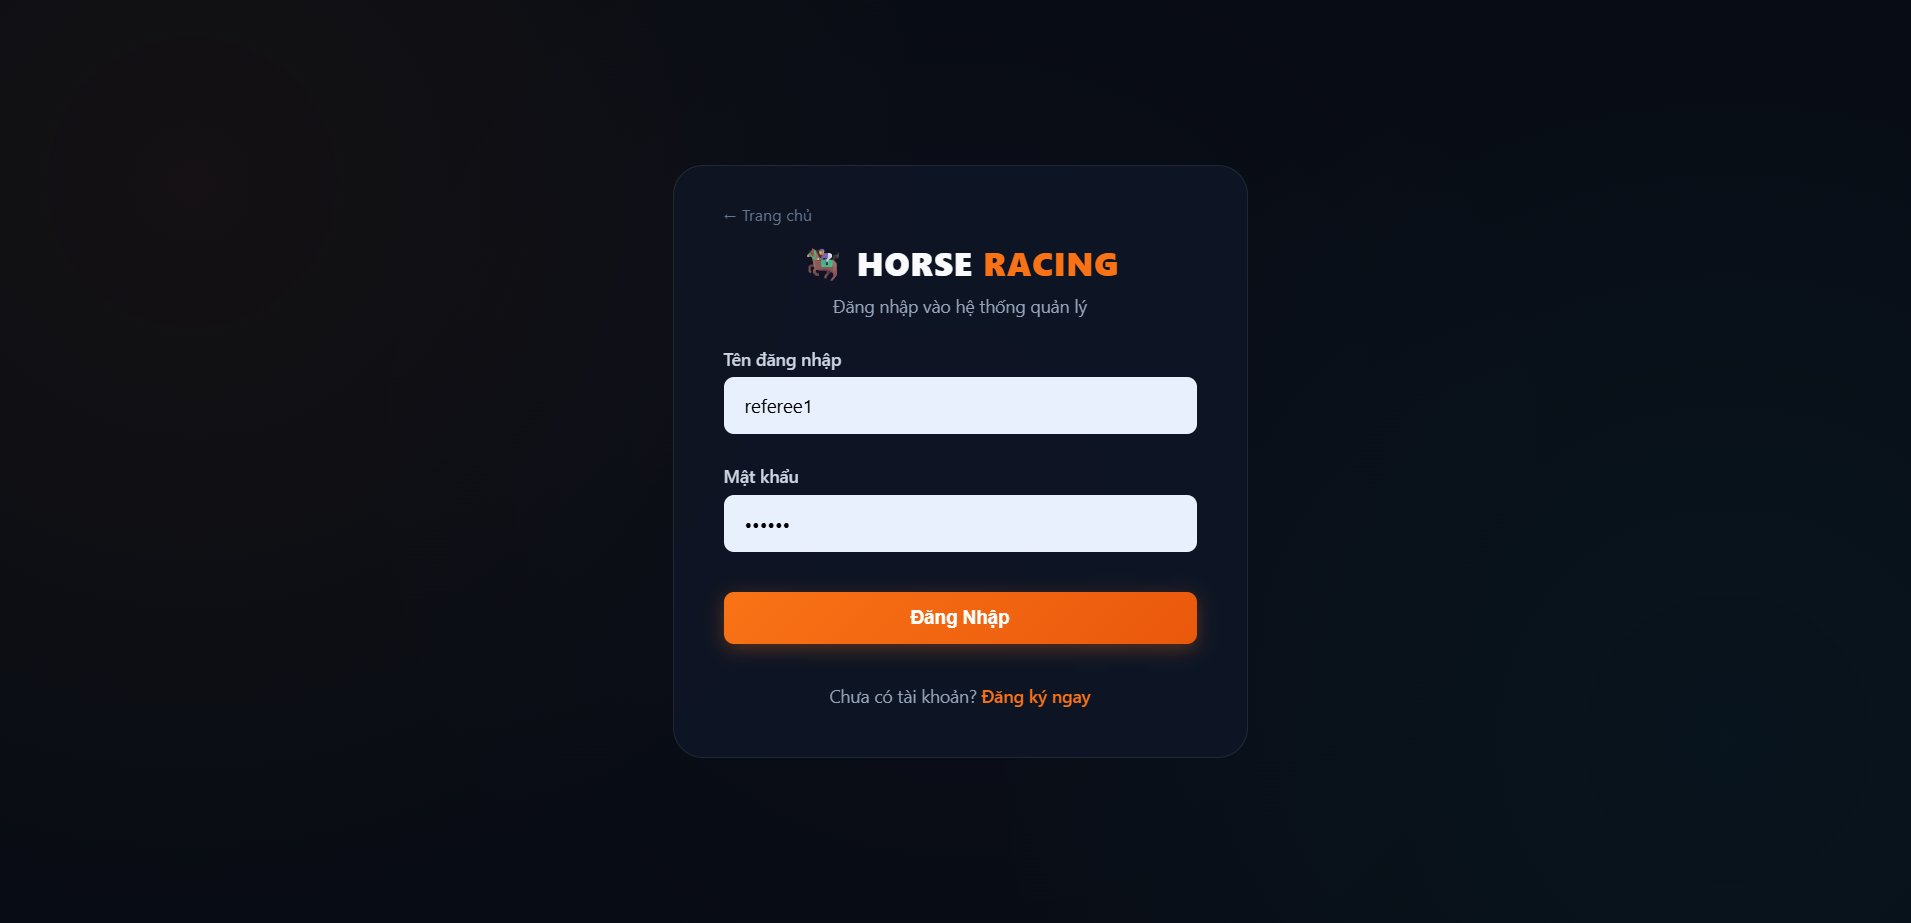
\includegraphics[width=0.7\textwidth]{figures/web_application/referee/Login.png}
    \caption{Referee Login}
\end{figure}

% ===================================================

\subsubsection{Assigned Race List}

\textbf{Role:} Race Referee

\begin{itemize}
    \item \textbf{Function trigger:} Select ``Tran dua phan cong''.

    \item \textbf{Function description:}
    \begin{itemize}
        \item \textbf{Purpose:}
        \begin{enumerate}
            \item View all races assigned to the referee for supervision.
            \item Navigate to race inspection and result entry actions.
        \end{enumerate}

        \item \textbf{Data processing:}
        \begin{enumerate}
            \item Retrieve races assigned to the current referee.
            \item Retrieve race details including time, distance, track condition, and number of participants.
            \item Retrieve current race status.
            \item Display available action buttons based on race status.
        \end{enumerate}
    \end{itemize}

    \item \textbf{Function details:}
    \begin{itemize}
        \item Display race name, scheduled time, distance, and track condition.
        \item Display the number of participating horses.
        \item Display current race status (e.g., SCHEDULED, COMPLETED).
        \item Provide ``Kiem tra duong dua'' and ``Nhap ket qua'' buttons for scheduled races.
        \item Provide ``Sua ket qua'' button for completed races.
    \end{itemize}
\end{itemize}

\textbf{Screen layout:}

\begin{figure}[H]
    \centering
    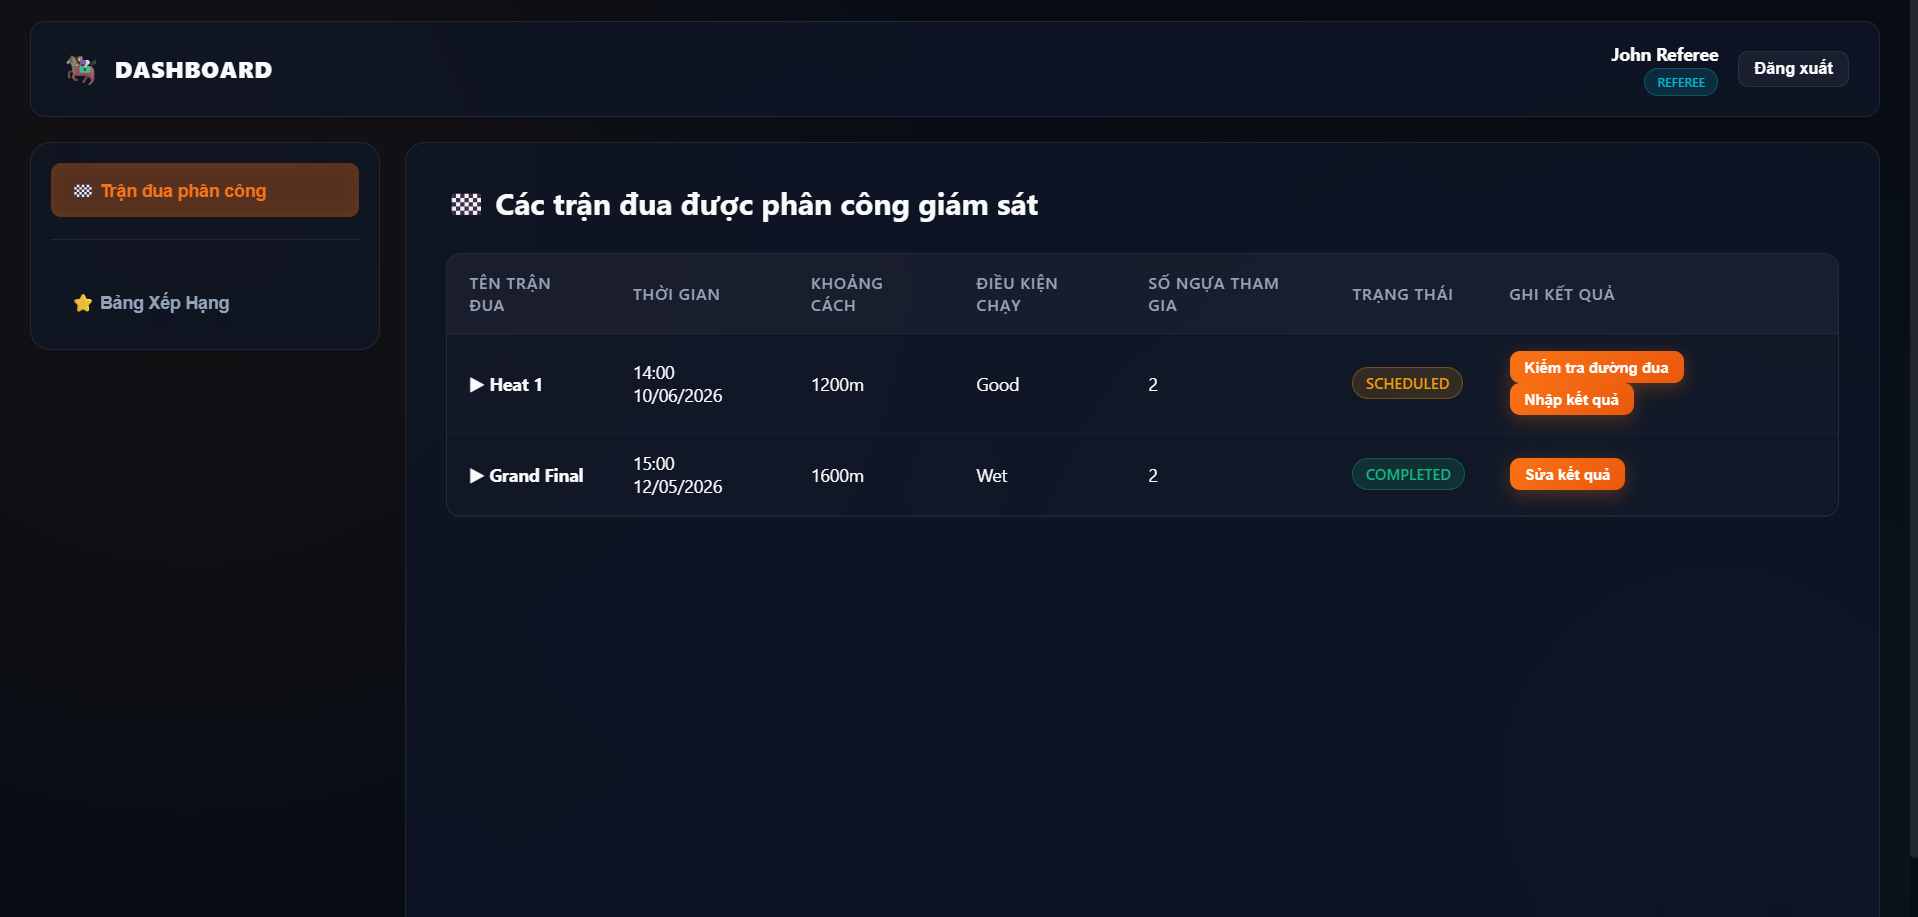
\includegraphics[width=\textwidth]{figures/web_application/referee/Assigned_Race_List.png}
    \caption{Assigned Race List}
\end{figure}

% ===================================================

\subsubsection{Race Inspection}

\textbf{Role:} Race Referee

\begin{itemize}
    \item \textbf{Function trigger:} Select ``Kiem tra duong dua'' on a scheduled race.

    \item \textbf{Function description:}
    \begin{itemize}
        \item \textbf{Purpose:}
        \begin{enumerate}
            \item Record pre-race track and environmental conditions.
            \item Assess horse health and fitness before the race.
        \end{enumerate}

        \item \textbf{Data processing:}
        \begin{enumerate}
            \item Enter current weather conditions.
            \item Enter track surface condition.
            \item Enter horse health assessment notes.
            \item Submit the inspection report to the system.
        \end{enumerate}
    \end{itemize}

    \item \textbf{Function details:}
    \begin{itemize}
        \item Input field for weather (e.g., Sunny, Rainy).
        \item Input field for track condition (e.g., Good, Wet, Muddy).
        \item Text area for horse health assessment.
        \item ``Gui bao cao kiem tra'' button to submit the inspection report.
        \item ``Huy'' button to cancel without saving.
    \end{itemize}
\end{itemize}

\textbf{Screen layout:}

\begin{figure}[H]
    \centering
    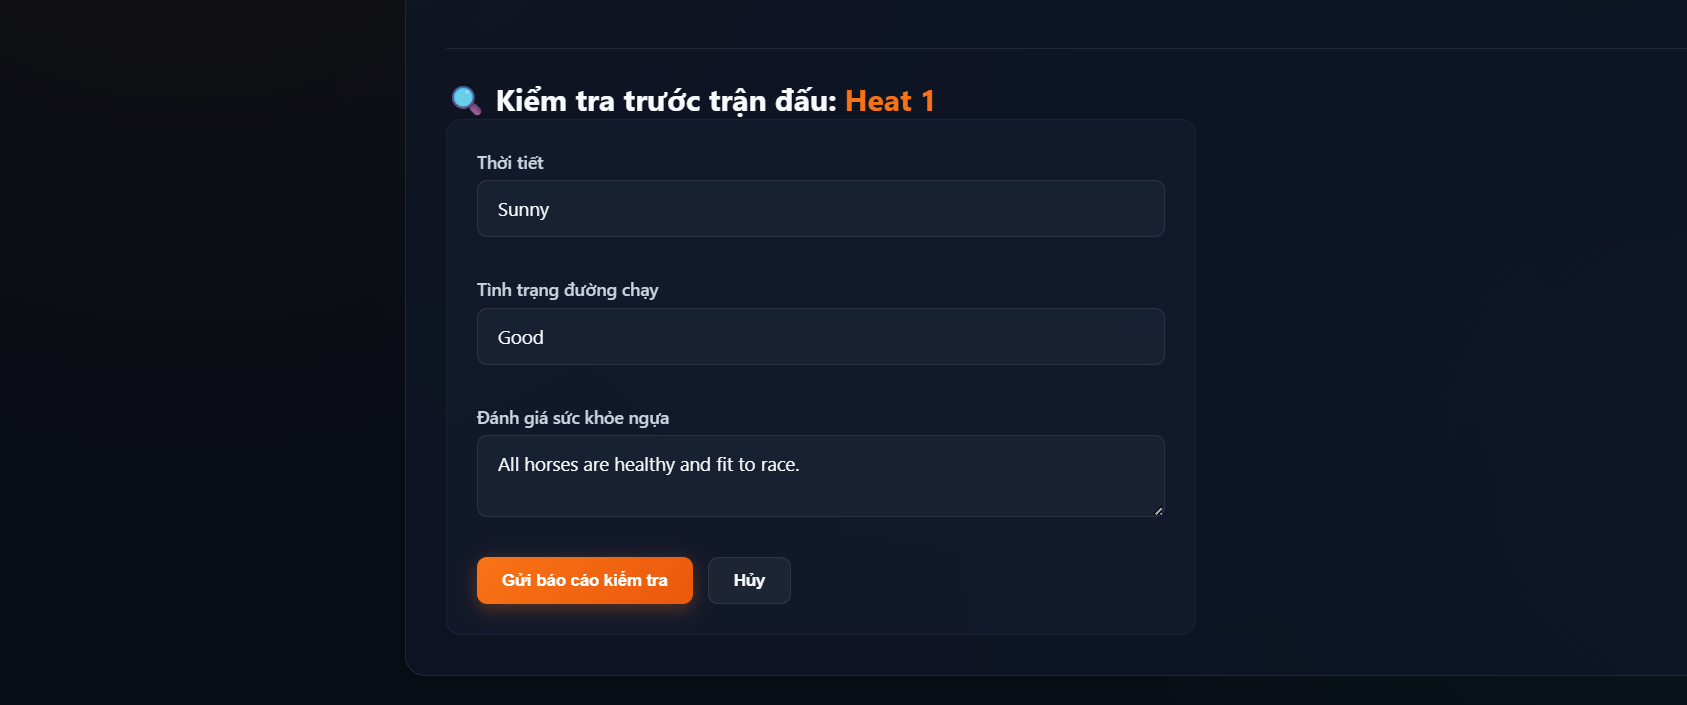
\includegraphics[width=0.85\textwidth]{figures/web_application/referee/Race_Inspection.png}
    \caption{Race Inspection}
\end{figure}

% ===================================================

\subsubsection{Input Result Form}

\textbf{Role:} Race Referee

\begin{itemize}
    \item \textbf{Function trigger:} Select ``Nhap ket qua'' on a scheduled race.

    \item \textbf{Function description:}
    \begin{itemize}
        \item \textbf{Purpose:}
        \begin{enumerate}
            \item Record finishing positions and scores for each participating horse.
            \item Add race notes or remarks for each horse.
        \end{enumerate}

        \item \textbf{Data processing:}
        \begin{enumerate}
            \item Retrieve the list of participating horses for the selected race.
            \item Enter finishing position (Hang ve dich) for each horse.
            \item Enter bonus/penalty points (Diem cong/tru) for each horse.
            \item Enter optional race notes (Ghi chu) for each horse.
            \item Save the result to the system.
        \end{enumerate}
    \end{itemize}

    \item \textbf{Function details:}
    \begin{itemize}
        \item Display each participating horse by name.
        \item Input field for finishing position per horse.
        \item Input field for bonus/penalty score adjustment per horse.
        \item Optional text field for race notes per horse.
        \item ``Luu ket qua cuoc dua'' button to save results.
        \item ``Huy'' button to cancel without saving.
    \end{itemize}
\end{itemize}

\textbf{Screen layout:}

\begin{figure}[H]
    \centering
    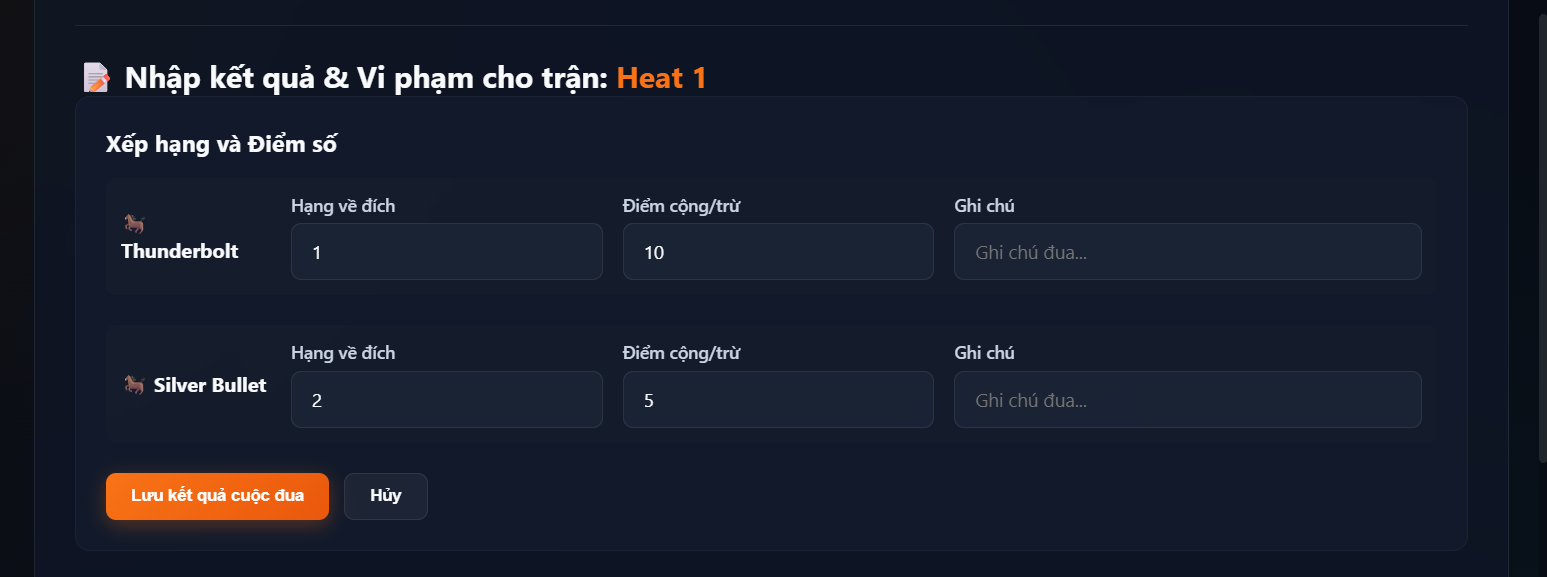
\includegraphics[width=\textwidth]{figures/web_application/referee/Input_Result_Form.png}
    \caption{Input Result Form}
\end{figure}

% ===================================================

\subsubsection{Violation Report}

\textbf{Role:} Race Referee

\begin{itemize}
    \item \textbf{Function trigger:} Access violation reporting within the result entry workflow.

    \item \textbf{Function description:}
    \begin{itemize}
        \item \textbf{Purpose:}
        \begin{enumerate}
            \item Document rule violations observed during the race.
            \item Apply appropriate penalties to the offending horse.
        \end{enumerate}

        \item \textbf{Data processing:}
        \begin{enumerate}
            \item Select the offending horse from the race participant list.
            \item Enter a description of the violation.
            \item Select the penalty type (e.g., Canh cao -- Warning, Phat tien -- Fine, Cam thi dau -- Disqualification).
            \item Enter the fine amount if applicable.
            \item Submit the violation report.
        \end{enumerate}
    \end{itemize}

    \item \textbf{Function details:}
    \begin{itemize}
        \item Dropdown to select the violating horse.
        \item Text area for violation description.
        \item Dropdown for penalty type selection.
        \item Numeric input for fine amount.
        \item ``Bao cao vi pham'' button to submit the report.
    \end{itemize}
\end{itemize}

\textbf{Screen layout:}

\begin{figure}[H]
    \centering
    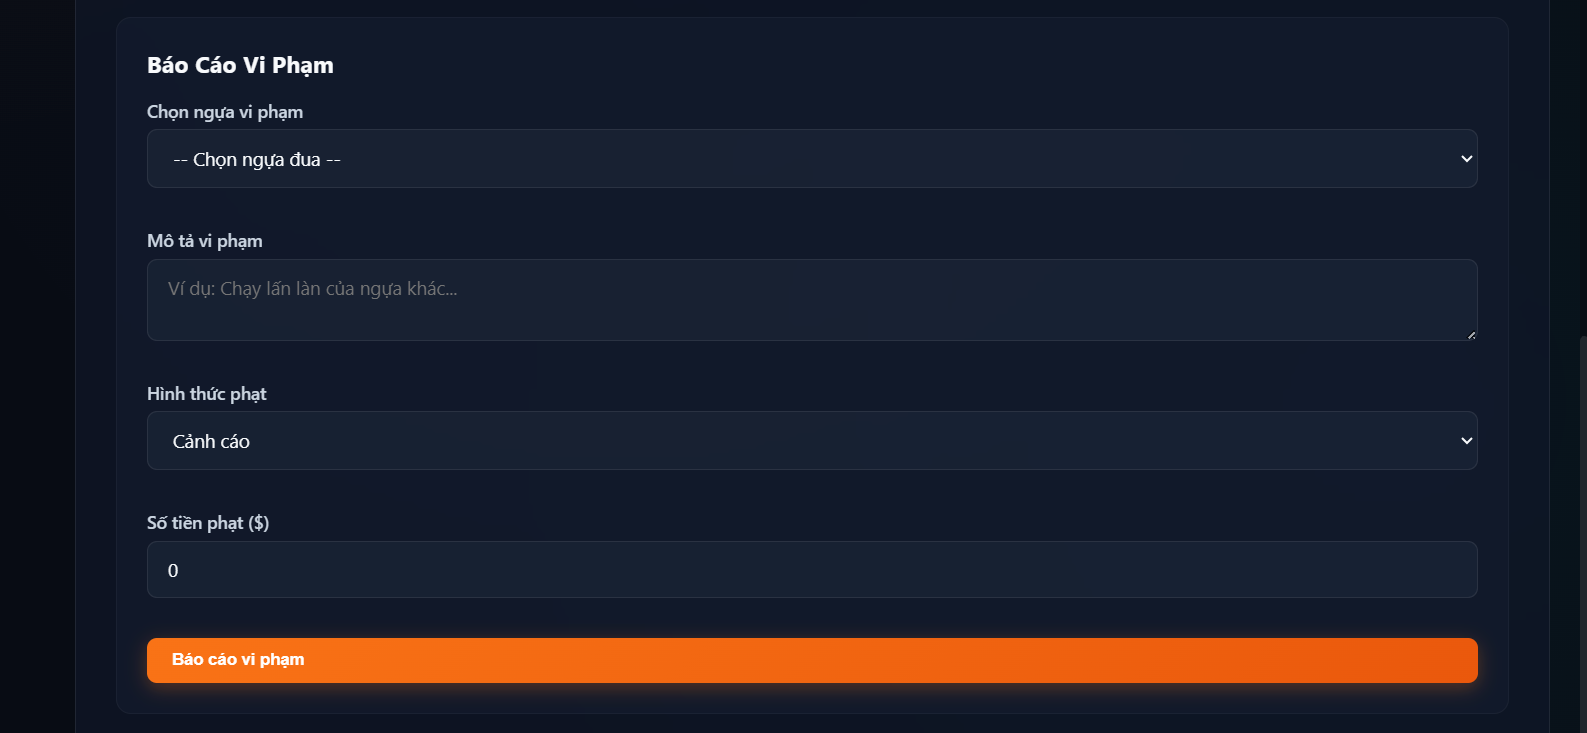
\includegraphics[width=\textwidth]{figures/web_application/referee/Violation_Report.png}
    \caption{Violation Report}
\end{figure}

% ===================================================

\subsubsection{Result Confirmed}

\textbf{Role:} Race Referee

\begin{itemize}
    \item \textbf{Function trigger:} Administrator approves the submitted result; referee views the updated race list.

    \item \textbf{Function description:}
    \begin{itemize}
        \item \textbf{Purpose:}
        \begin{enumerate}
            \item Display confirmed race results after administrator approval.
            \item Allow the referee to resubmit corrected results if needed.
        \end{enumerate}

        \item \textbf{Data processing:}
        \begin{enumerate}
            \item Retrieve updated race status from the system.
            \item Display the race with status RESULTS\_ENTERED or COMPLETED.
            \item Provide result confirmation and editing options based on status.
        \end{enumerate}
    \end{itemize}

    \item \textbf{Function details:}
    \begin{itemize}
        \item Display race list with updated statuses after administrator review.
        \item ``Xac nhan ket qua chinh thuc'' button available for races with RESULTS\_ENTERED status.
        \item ``Sua ket qua'' button available for COMPLETED races requiring correction.
        \item ``Nhap ket qua'' button to re-enter results if necessary.
    \end{itemize}
\end{itemize}

\textbf{Screen layout:}

\begin{figure}[H]
    \centering
    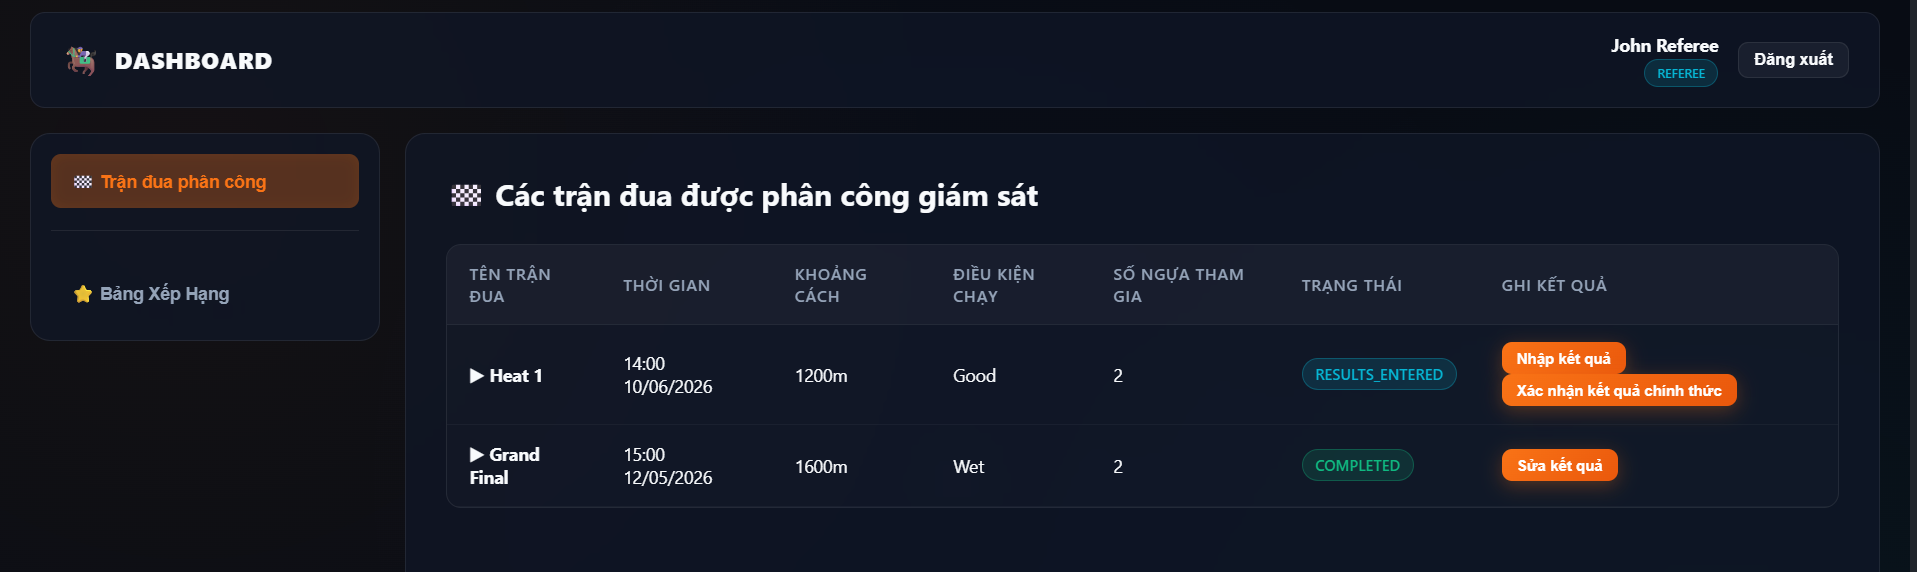
\includegraphics[width=\textwidth]{figures/web_application/referee/Result_Confirmed.png}
    \caption{Result Confirmed}
\end{figure}

% ===================================================

\subsubsection{Ranking Board}

\textbf{Role:} Race Referee

\begin{itemize}
    \item \textbf{Function trigger:} Select ``Bang Xep Hang''.

    \item \textbf{Function description:}
    \begin{itemize}
        \item \textbf{Purpose:}
        \begin{enumerate}
            \item View official tournament standings for horses, jockeys, and spectators.
            \item Filter rankings by tournament.
        \end{enumerate}

        \item \textbf{Data processing:}
        \begin{enumerate}
            \item Retrieve horse and jockey accumulated scores from confirmed race results.
            \item Retrieve spectator prediction scores.
            \item Filter rankings by selected tournament.
            \item Display ranked lists for each category.
        \end{enumerate}
    \end{itemize}

    \item \textbf{Function details:}
    \begin{itemize}
        \item Toggle tabs between ``Ngua \& Jockey'' and ``Khan gia xuat sac'' views.
        \item Filter rankings by tournament (e.g., All, Summer Championship 2026, Spring Derby 2026).
        \item Display horse ranking table with position, horse name, and accumulated points.
        \item Display jockey ranking table with position, jockey name, and accumulated points.
    \end{itemize}
\end{itemize}

\textbf{Screen layout:}

\begin{figure}[H]
    \centering
    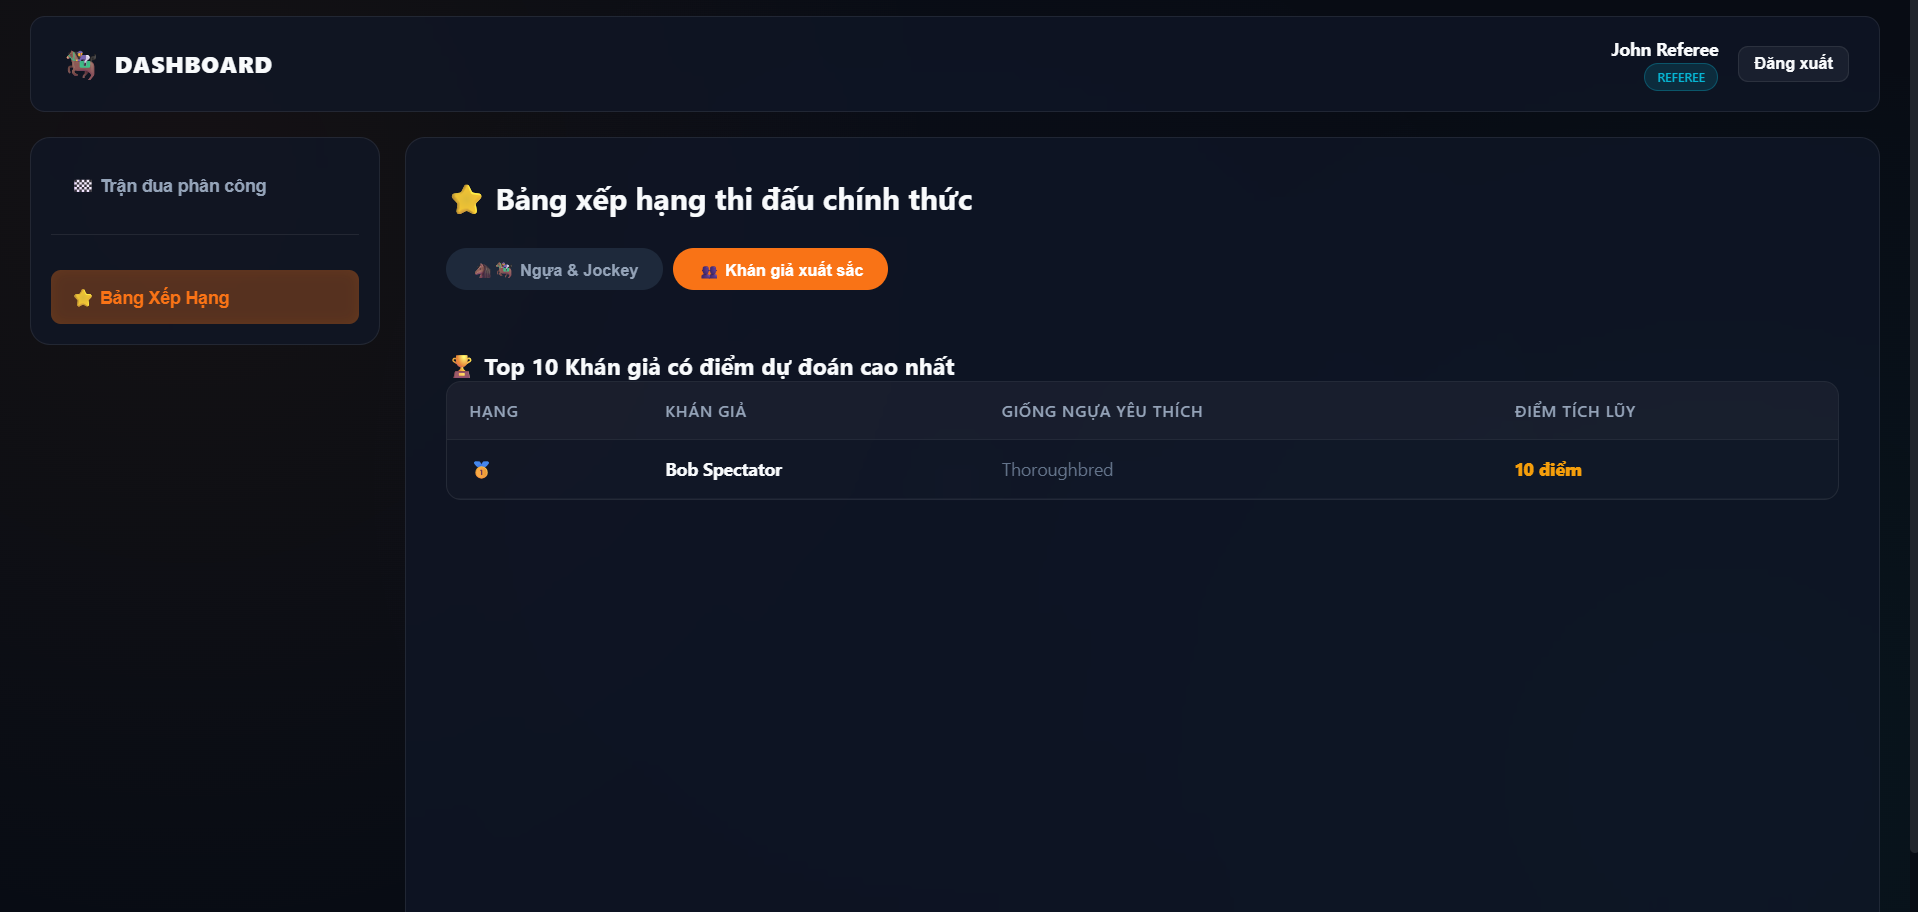
\includegraphics[width=\textwidth]{figures/web_application/referee/Ranking_Board.png}
    \caption{Ranking Board}
\end{figure}

% ===================================================

\subsubsection{Leaderboard}

\textbf{Role:} Race Referee

\begin{itemize}
    \item \textbf{Function trigger:} Select the ``Khan gia xuat sac'' tab within the Ranking Board.

    \item \textbf{Function description:}
    \begin{itemize}
        \item \textbf{Purpose:}
        \begin{enumerate}
            \item View the top spectators ranked by their prediction accuracy.
            \item Recognize outstanding spectator engagement.
        \end{enumerate}

        \item \textbf{Data processing:}
        \begin{enumerate}
            \item Retrieve spectator prediction scores from the system.
            \item Sort spectators by accumulated prediction points in descending order.
            \item Display the top 10 spectators.
        \end{enumerate}
    \end{itemize}

    \item \textbf{Function details:}
    \begin{itemize}
        \item Display ranking position, spectator name, preferred horse breed, and accumulated points.
        \item Highlight top-ranked spectator with a medal icon.
        \item Read-only view accessible to the referee for reference.
    \end{itemize}
\end{itemize}

\textbf{Screen layout:}

\begin{figure}[H]
    \centering
    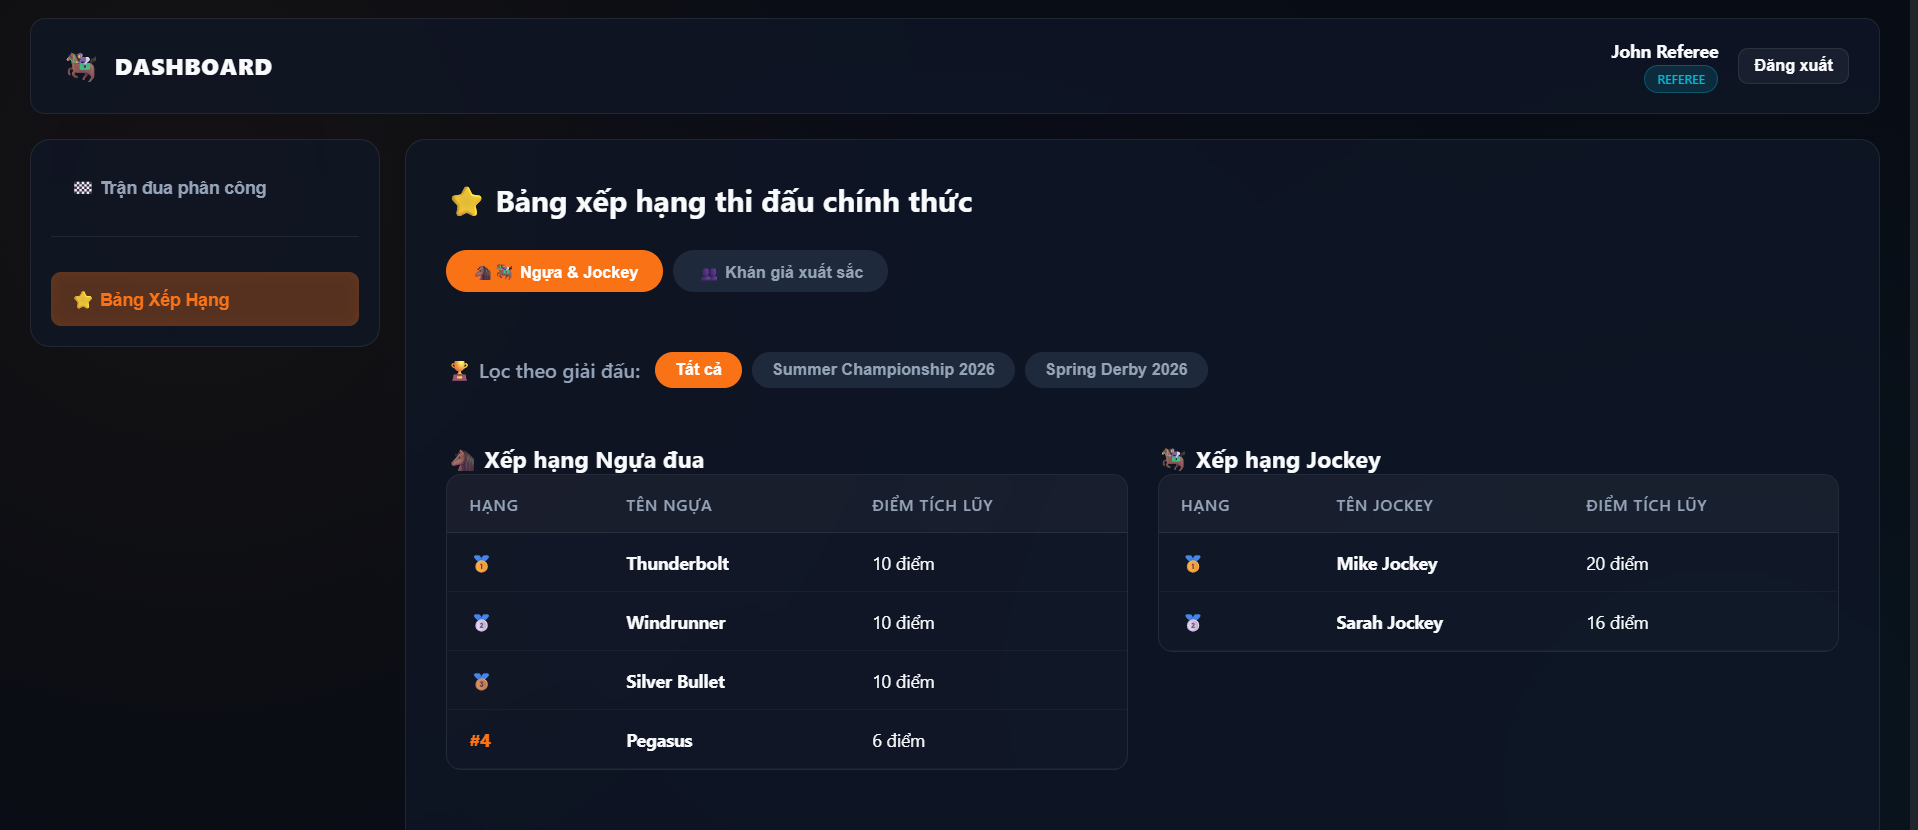
\includegraphics[width=\textwidth]{figures/web_application/referee/Leaderboard.png}
    \caption{Leaderboard}
\end{figure}
